\section{A Discrete Version}
\label{sec:discrete}

In this section, we use the Gauss-Bonnet theorem to derive
a definition of discrete curvature. We discuss how discrete curvature
is used to improve meshes that are generated by scanning.
We then prove a discrete version of the Gauss-Bonnet theorem.

Consider a triangulated polygonal surface $S$ with boundary $\partial(S)$.
The boundary is a one dimensional piecewise linear curve in $\R^3.$
As with polygons in the plane, at each vertex $v\in \partial(S)$ 
we have an exterior angle.

The interior angle might consist of many triangles.
Let $F_v$  denote the set of faces incident to $v$ and let
$\alpha_f$ denote the angle in face $f$ at $v$.
The \EMPH{discrete geodesic curvature}
of $v$  is
$$k_{g}(v)= \pi-\sum_{f\in F_v}\epsilon_f.$$
See \figref{discrete-geodesic} for an illustration.
Notice that if $v$ lies on a straight line, then $\sum_{i}\epsilon_f=\pi$
and the curvature is zero as we would expect.


\begin{figure}[htb]
\centering
	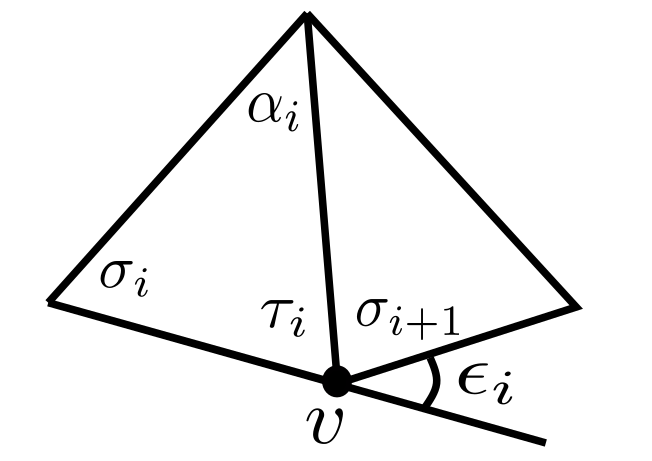
\includegraphics[width=.3\textwidth]{curvature/discrete-geodesic}
	\caption{The discrete geodesic curvature at a vertex $v$ on the boundary
	of a surface is given by the exterior angle $\epsilon$.}
	\label{fig:discrete-geodesic}
\end{figure}

How should be define discrete Gaussian curvature?
At every non-vertex point on a polygonal surface, the continuous Gaussian curvature
is zero and at every vertex it is undefined.
We can use the intuitive definition of discrete geodesic curvature and the Gauss-Bonnet
theorem to give a definition for discrete Gaussian curvature.

Consider removing the neighborhood around a vertex $v$ consisting
of the faces incident to $v$ and the edges and vertices of these faces call
this $N(v)$.
Using the variable names given in \figref{discrete-geodesic},
the total geodesic cuvature
$$=$$

\begin{align}
\int_{\partial N(v)} kg ds &=\sum_i \pi -(\tau_i+\sigma_{i+1})\nonumber  \\
       &=\sum_i \pi -(\tau_i+\sigma_{I}) \nonumber  \\
       &=\sum_i \alpha_i. \nonumber 
\end{align}
Where the second equality comes from the boundary being a circle and reorganizing the sum.
Topologically, this neighborhood is a disk and $\chi(N(v))=1$
so the Gauss-Bonnet theorem tells us that 
the discrete Gaussian curvature at a vertex is
\begin{definition}[Discrete Gaussian curvature\footnote{Discrete Gaussian curvature
is also called the \emph{angle defect} at a vertex}]\label{def:discrete-curvature-vertex}

$$K(v)=\int_{N(v)}K da=2\pi-\sum_i \alpha_i.$$

\end{definition}

Recall, that when we considered the curvature at a vertex on a polygon in the plane
in the theorem of turning tangents, \thmref{simple-bonnet}, we have two parts depending on
weather we use the interior or the exterior angles at each vertex.
We can do a similar thing with the discrete Gaussian curvature at a vertex on a surface,
instead of considering the angles of the faces incident to a vertex $v$, we can consider
the complementary angle. The complementary angle is shown in \figref{switcheroo}. 
If we let $n$ be the number of faces
incident to $v$, the formula for the discrete curvature then becomes
\begin{equation}\label{eqn:discrete-curvature-complement-angle}
K(v)=2\pi - \sum_{i=1}^n (\pi - \xi_i)=(2-n)\pi +\sum_{i=1}^n \xi_i.
\end{equation}
By \eqnref{sphere-area}, this is the area of the polygon on the sphere with interior
angles $\xi_1, \xi_2,\ldots \xi_n.$
Geometrically, this angle be seen in \figref{switcheroo}.
If we project the normal vectors on each face onto a sphere and
connect these points with great arcs to create a polygon on the sphere with interior angles
$\xi_1, \xi_2,\ldots \xi_n.$
We have a geometric representation of discrete
Gaussian curvature as the area on the unit 
sphere bounded by a spherical polygon whose vertices are the unit normals of 
the faces around $v$. An example is shown in \figref{discrete-curvature}.

\begin{figure}[htb]
\centering
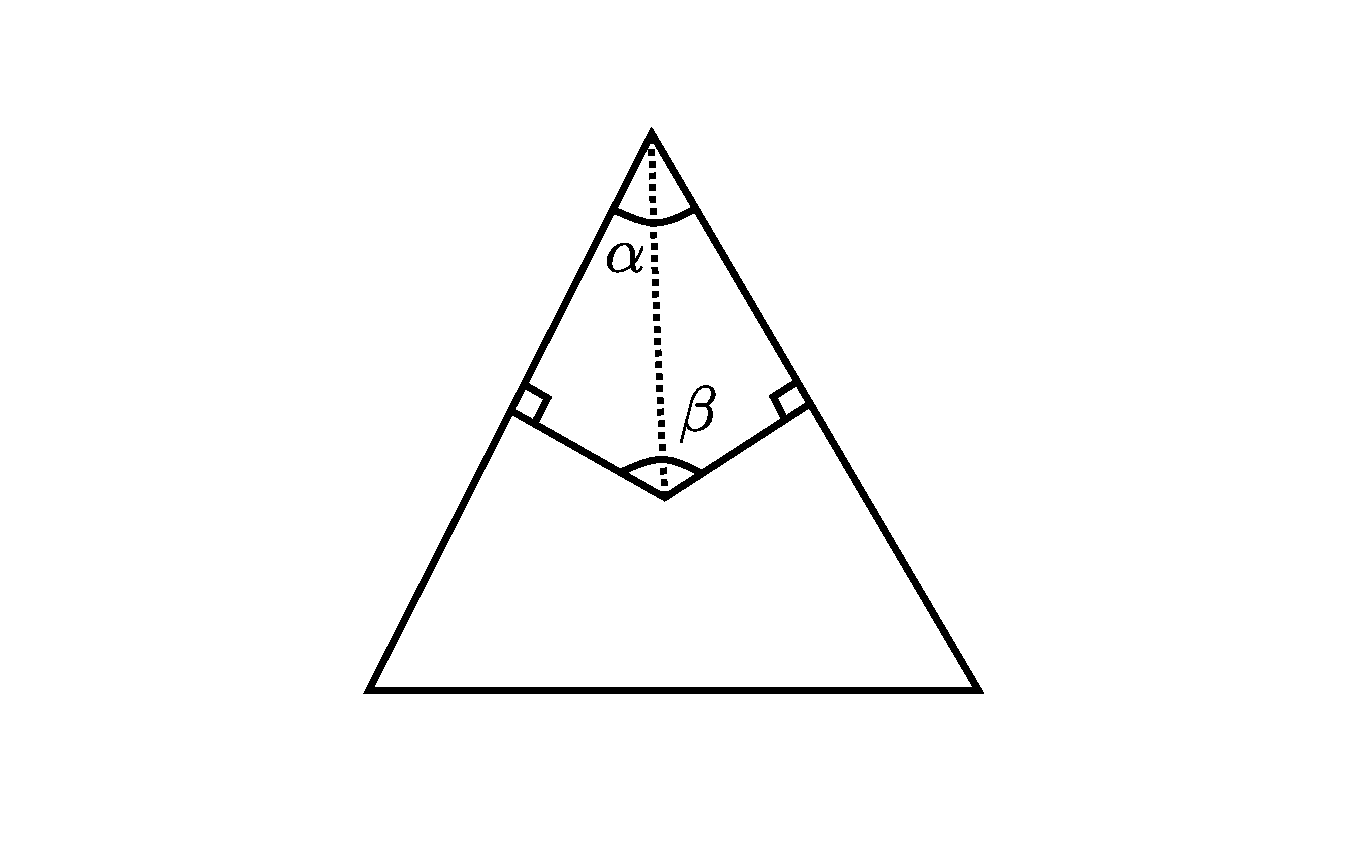
\includegraphics[width=.25\textwidth]{background/switch-angles}
\caption{The relationship between the angles incident to a vertex and
its complementary angle.}
\label{fig:switcheroo}
\end{figure}





\begin{figure}[htb]
\centering
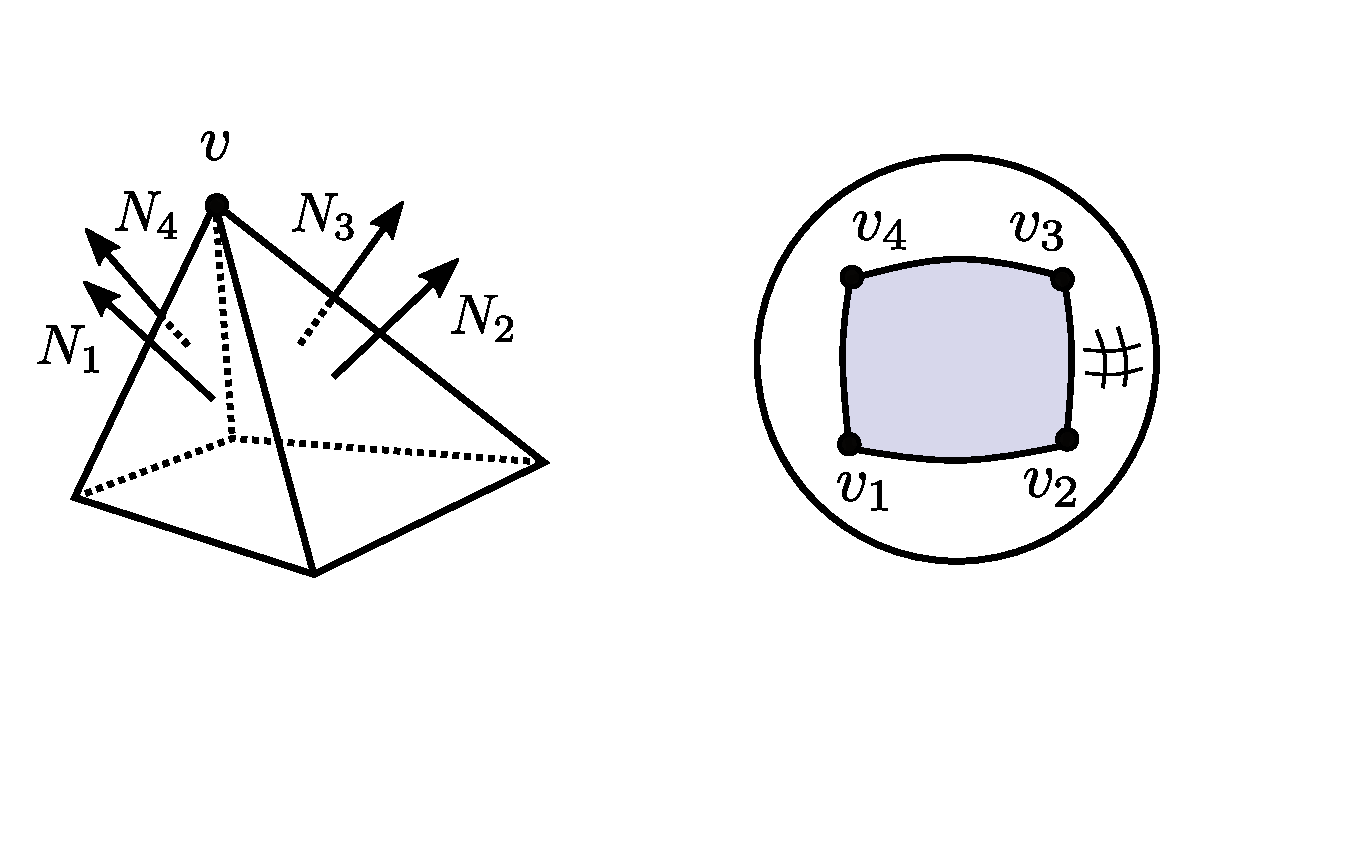
\includegraphics[width=.5\textwidth]{curvature/discrete-curvature}
\caption{Consider the vertex $v$ in the figure on the left. The curvature of $v$
is the area on the sphere shown on the right. We rotated the sphere
in order to see the entire polygon.}
\label{fig:discrete-curvature}
\end{figure}







Combining the above definitions  we have

\begin{theorem}[The Discrete Gauss-Bonnet Theorem] \label{thm:g-b-d}

If $S$ is a triangulated surface with  boundary $\partial S$ then
$$\sum_{v\in V_{int}} K(v) + \sum_{v\in V_{\partial S}} k_g(v) = 2\pi \chi(S)$$
where $K(v)$ is the discrete Gaussian curvature
of a vertex, $k_g(g)$ is the discrete geodesic curvature,  and
$\chi$ is the Euler characteristic.
\end{theorem}



\section{Removing Noise From A Scanned Object}
\label{sec:removing}



Meshes that are obtained by scanning real objects contain noise.
Most meshes that are generated by scanning require a complete
remeshing \cite{remeshing-2003}.
As a first step in remeshing, the curvature at each
vertex needs to be estimated.

In \cite{mmsb-2003}, Meyer et al., define the gaussian curvature operator
to estimate the curvature at each vertex. Their operator is 
based on a simple application of the Gauss-Bonnet theorem.
The central idea is to cut a disk around each vertex that does not contain
any other vertices. Then, all Gaussian curvature in the removed
disk is occurs at the vertex of interest.

We associate an area around each vertex$v$. 
For each triangle incident to $v$, if the interior 
angle at $v$ is non-obtuse, mark the circumcenter of the triangle
and if the interior angle is obtuse, make the mid point of the edge
opposite of $v$. See \figref{mixed-area} for an illustration.
Denote the area of this polygon by $A_m.$


\begin{figure}[htb]
\centering
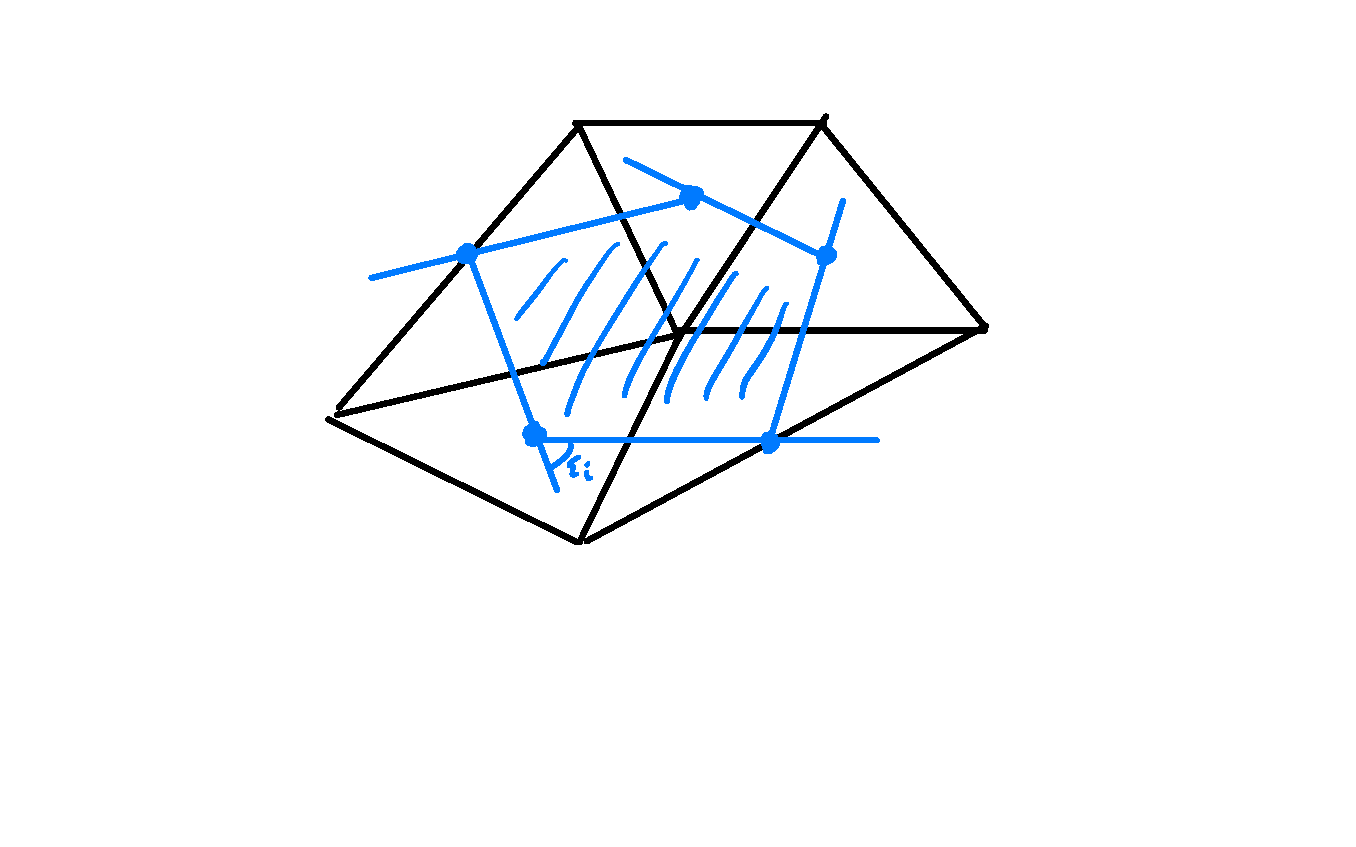
\includegraphics[width=.3\textwidth]{meshes/mixed-area}
\caption{The area $A_m$ associated with a vertex $v$.}
\label{fig:mixed-area}
\end{figure}


Then, since we are considering a closed two-disk $A$ we have $\chi(A)=1$.
Let $F_v$ denote the number of faces incident to $v$, 
then by the Gauss-Bonnet theorem we have

$$\int \int_{A_m}K dA +\sum_i^{F_v} \epsilon_i=2\pi$$
where the sum is over the faces incident to $v$.
The Gaussian curvature operator at a vertex $v$ is defined
to be
$$K(v)=\left( 2\pi -\sum_i^{F_v}\epsilon_i\right)/ A_m.$$

The experiments in \cite{mmsb-2003} found that the average
percent error did not exceed $1.3\%$ when using this operator.



\subsection{A Combinatorial Proof}
\label{sec:proof}


We present a proof of the Gauss-Bonnet theorem similar to the proof given by Upadhyay \cite{upadhyay2015}.
First, we consider the case where our surface does not have a boundary.
We then extend this case to surfaces with boundary.
\begin{theorem}[Discrete surfaces without boundary]\label{thm:g-b-discete-bdy}
For a triangulated surface $S$ without boundary
$$\sum_{v\in V} K(v)=2\pi \chi(S)$$
where $K(v)$ is the discrete curvature.
\end{theorem}

\begin{proof}

For each vertex $v$ in $S$,
let $deg(v)$ denote the number of edges incident to $v$, let $\alpha_1,\alpha_2,\ldots,\alpha_{\deg{(v)}}$ denote the angles
containing $v$ and let $\xi_i=\pi-\alpha_i$ for each $i$.
By \eqnref{discrete-curvature-complement-angle}, 
the discrete Gaussian curvature at a $v$ is
 $$K(v)=(2-\deg{(v)})\pi +\sum_{i=1}^{\deg{(v)}} \xi_i.$$
Summing over all vertices in $S$ gives
$$\sum_{v\in V} K(v)=\sum_{v\in V}2\pi - \sum_{v\in V}\deg{(v)}\pi+\sum_{v\in V}\sum_{i=1}^{\deg{(v)}} \xi_i.$$
The first term on the right hand side is $2\pi |V|$. Each edge is incident with two vertices, so the second term is $2\pi |E|$. 
In the third term, we rewrite $\xi_i$ as $\pi-\alpha_i$.

$$ \sum_{v\in V}\sum_{i=1}^{\deg{(v)}} \beta_i= \sum_{v\in V}\sum_{i=1}^{\deg{(v)}} (\pi-\alpha_i).$$
We can reorganize this sum as follows, instead of summing the angles around each vertex we can sum the angles in each face.
Each angle in $S$ is still being counted exactly once. 
Since each face is a triangle, this gives
$$\sum_{v\in V}\sum_{i=1}^{\deg{(v)}} (\pi-\alpha_i)=\sum_{f\in F}\sum_{i=1}^3(\pi-\alpha_i).$$
Since each face is a triangle the sum of the three angles is $\pi$,
so $\sum_{i=1}^3(\pi-\alpha_i)=3\pi-\pi=2\pi.$
Thus, $$\sum_{v\in V} K(v)=2\pi |V|-2\pi |E|+2\pi |F|=2\pi \chi(S)$$ as desired.
\end{proof}

Next, we extend the above proof to the case where $S$ has a boundary
by gluing a copy of $S$ to itself along the boundary.

\begin{theorem}[Discrete surfaces without boundary]\label{thm:g-b-discete}
For a combinatorial surface $S$ with boundary

$$\sum_{v\in S_{\text{int}}} K(v)+\sum_{v\in\partial S}k_g(v)=2\pi \chi(S)$$
where $K(v)$ is the discrete curvature and $k_g(v)$ is the discrete geodesic curvature.
\end{theorem}

\begin{proof}
Take a copy of $S$ and attach it to itself along the boundary.
This creates the surface $2S$ without boundary. Notice,
when we copy $S$ we create two copies of the boundary, and when
we glue we remove one copy of the boundary.
Thus, $$\chi(2S)=2\chi(S)-\chi(\partial S).$$
Since, $\partial S$ is piecewise linear the number of vertices and
edges are equal and there are no faces, so $\chi(\partial S)=0$
and 

\begin{equation} \label{eqn:glue}
\chi(2S)=2\chi(S).
\end{equation}
For $v$ a vertex on the boundary, $k_g(v)$ is half
the discrete Gaussian curvature of $v$ in $2S.$
Thus,

$$\sum_{v\in 2S}K(v)=2\left(\sum_{v\in S_{\text{int}}}K(v)+\sum_{v\in \partial S} k_g(v)\right) =2\pi  \chi(2S).$$
Applying \eqnref{glue},

$$\sum_{v\in S}K(v)+\sum_{v\in \partial S} k_g(v)=2\pi  \chi(S)$$
as desired.

\end{proof}